% ****** Start of file templateForReport.tex ******

% TeX'ing this file requires that you have all prerequisites
% for REVTeX 4.2 installed
%
% See the REVTeX 4 README file
% It also requires running BibTeX. The commands are as follows:
%
%  1)  latex templateForReport.tex
%  2)  bibtex templateForReport
%  3)  latex templateForReport.tex
%  4)  latex templateForReport.tex
%
\documentclass[%
 reprint,
%superscriptaddress,
%groupedaddress,
%unsortedaddress,
%runinaddress,
%frontmatterverbose,
%preprint,
%showpacs,preprintnumbers,
%nofootinbib,
%nobibnotes,
%bibnotes,
 amsmath,amssymb,
 aps,
%pra,
%prb,
%rmp,
%prstab,
%prstper,
%floatfix,
]{revtex4-2}

\usepackage{graphicx}% Include figure files
\usepackage{dcolumn}% Align table columns on decimal point
\usepackage{bm}% bold math
\usepackage{todonotes}
\usepackage{siunitx}
\usepackage{subcaption}
\usepackage{mwe}
\usepackage{hyperref}

%\usepackage{hyperref}% add hypertext capabilities
%\usepackage[mathlines]{lineno}% Enable numbering of text and display math
%\linenumbers\relax % Commence numbering lines

%\usepackage[showframe,%Uncomment any one of the following lines to test
%%scale=0.7, marginratio={1:1, 2:3}, ignoreall,% default settings
%%text={7in,10in},centering,
%%margin=1.5in,
%%total={6.5in,8.75in}, top=1.2in, left=0.9in, includefoot,
%%height=10in,a5paper,hmargin={3cm,0.8in},
%]{geometry}

\begin{document}

\title{Advanced Methods of Data Analysis: Normalizing Flows}% Force line breaks with \\
%\thanks{A footnote to the article title}%

\author{Leonhard Moske}
%\author{Second Author}
 %\email{Second.Author@institution.edu}

%\author{Charlie Author}
% \homepage{http://www.Second.institution.edu/~Charlie.Author}

%\author{Delta Author}

\date{\today}% It is always \today, today,
             %  but any date may be explicitly specified

\begin{abstract}
%  An article usually includes an abstract, a concise summary of the work
%  covered at length in the main body of the article.
%  \begin{description}
%  \item[Usage]
%    Secondary publications and information retrieval purposes.
%  \item[Structure]
%    You may use the \texttt{description} environment to structure your abstract;
%    use the optional argument of the \verb+\item+ command to give the category of each item.
%  \end{description}

In this paper, a method named normalizing flows is utilized to construct density estimators for the purpose of classification. Normalizing flows are a class of transformation, which can be trained with gradient descend to estimate the distribution of data or to generate data in a toy model. The potential of this method is tested by classifying \textit{RR-Lyrae variable stars} of the \textit{AstroML RR-Lyrae variable stars data}-dataset.
Two different implementations of normalizing flows are tested for comparison.

\end{abstract}
\maketitle

%\tableofcontents

\section{Introduction}
Normalizing flows is a powerful method that utilizes the transformation of random variables for either density estimation or for generative sampling.

To demonstrate the functionality of normalizing flows we investigate the \textit{AstroML RR-Lyrae variable stars data}-dataset \cite{astroML} which contains a record of \textit{RR-Lyrae variable stars} \cite{Sesar_2009}. These are periodic variable stars, found in globular cluster, that serve as standard candles to measure extra galactic distances. The data was taken at the \textit{Sloan Digital Sky Survey (SDSS)}.
 The features provided are four intensities at different wavelength filters corresponding to the photometric system. The four features are: $\left\{u-g, g-r, r-i, i-z\right\}$, where $u$ is at $\SI{355}{nm}$, $g$ at \SI{468}{nm}, $r$ at \SI{616}{nm}, $i$ at \SI{748}{nm} and $z$ at \SI{893}{nm}, Figure~\ref{fig:filterResp}. The dataset contains background stars further named background and the \textit{RR-Lyrae variable stars}, which we are going to call signal. The number of background entries is \SI{92658}{} and of the signal \SI{483}{}.
 In figure \ref{fig:features} we see the features of signal and background and we can see that the features of the signal are grouped within the range of all feature values, making a classification easier. The \textit{Kolmogorov-Smirnov}-test validates this, because all features have scores higher than 0.75, see table \ref{tab:kolmogorov}.
 
 \begin{table}
 	\centering
 	\begin{tabular}{|l|l|}
 		\hline
		feature & score\\
		\hline
		$u-g$& 0.80\\
		$g-r$& 0.94\\
		$r-i$& 0.91\\
		$i-z$& 0.76\\
		\hline
 	\end{tabular}
 	\caption{Kolmogorov-Smirnov score of the four features \label{tab:kolmogorov}}
 \end{table}
 
 
 \begin{figure}[]
 	\centering
 	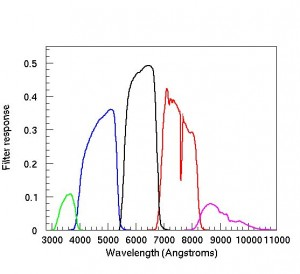
\includegraphics[width=0.4\textwidth]{figs/camera_filters-300x274.jpg}
 	\caption{ Filter response to different wavelengths of the \textit{SDSS}-camera. Form left to right the filters are: u, g, r, i and z. \cite{rgbSpec}
 		\label{fig:filterResp}
 	}
 \end{figure}
 
  \begin{figure*}
 	\centering
 	\begin{subfigure}[b]{0.4\textwidth}
 		\centering
 		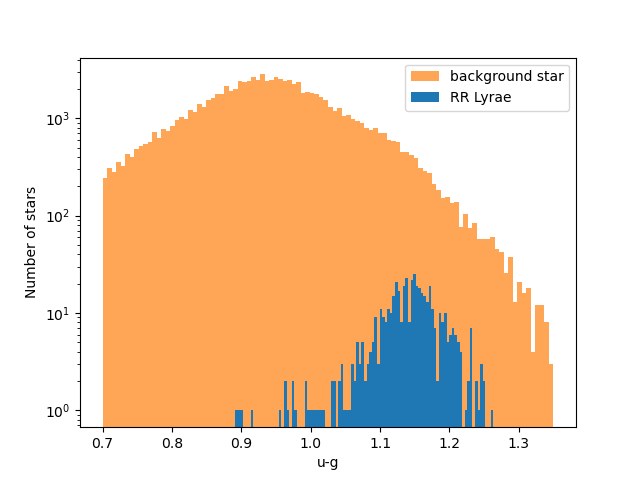
\includegraphics[width=\textwidth]{figs/hist_xData_feature0_labelSplit.png}
 		%\caption[feature $u-g$ of the data]%
 		%{{\small Network 1}}    
 		\label{fig:mean and std of net14}
 	\end{subfigure}
 	\hfill
 	\begin{subfigure}[b]{0.4\textwidth}  
 		\centering 
 		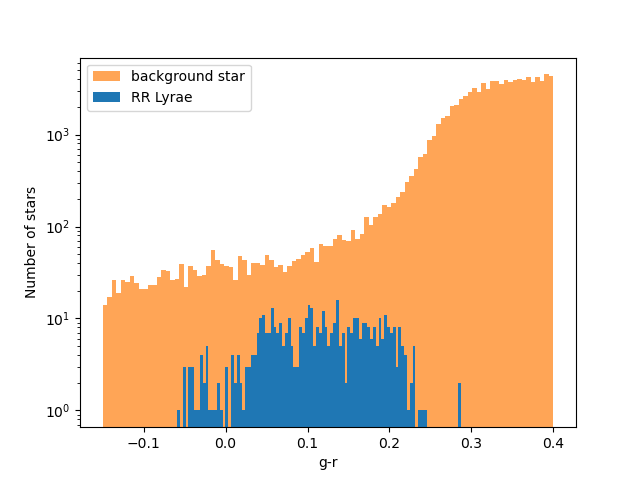
\includegraphics[width=\textwidth]{figs/hist_xData_feature1_labelSplit.png}
 		%\caption[]%
 		%{{\small Network 2}}    
 		\label{fig:mean and std of net24}
 	\end{subfigure}
 	\vskip\baselineskip
 	\begin{subfigure}[b]{0.4\textwidth}   
 		\centering 
 		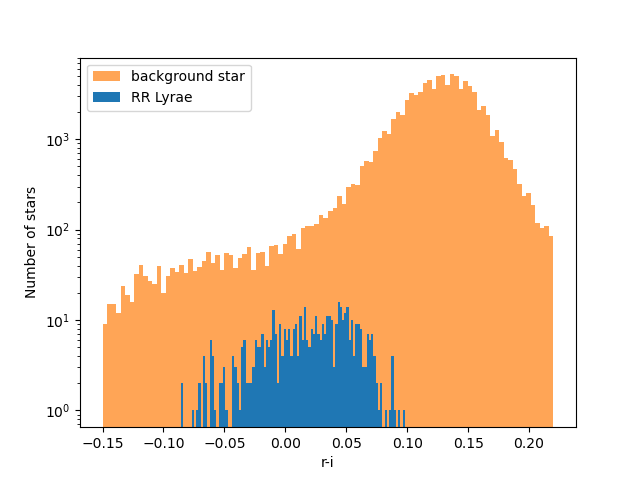
\includegraphics[width=\textwidth]{figs/hist_xData_feature2_labelSplit.png}
 		%\caption[]%
 		%{{\small Network 3}}    
 		\label{fig:mean and std of net34}
 	\end{subfigure}
 	\hfill
 	\begin{subfigure}[b]{0.4\textwidth}   
 		\centering 
 		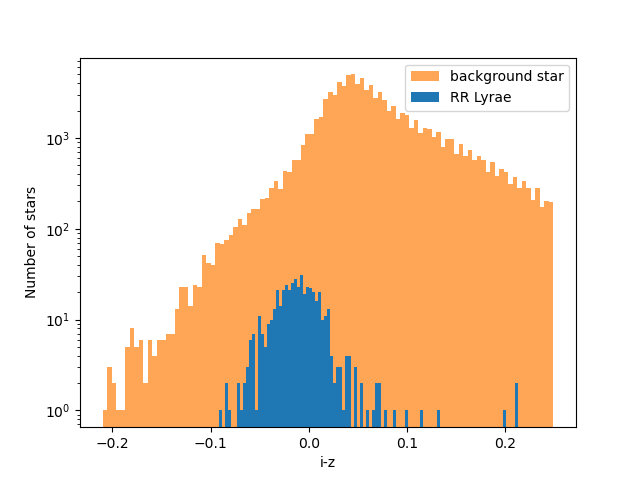
\includegraphics[width=\textwidth]{figs/hist_xData_feature3_labelSplit.png}
 		%\caption[]%
 		%{{\small Network 4}}    
 		\label{fig:mean and std of net44}
 	\end{subfigure}
 	\caption[ histograms of the features with the data split into background and signal ]
 	{\small histograms of the features with the data split into background and signal} 
 	\label{fig:features}
 \end{figure*}
 

\section{Theory}
\label{sec:theory 1}
To classify data into different categories (background and signal) using the density of these categories we have to evaluate the probability density distributions at the data and compare the result, i.e. choose the category with the highest probability. In this case we have only two categories (background named 0, signal named 1), thus we can use a test statistic like:
\begin{align*}
	t(\text{data}) = \ln(\frac{p(0|\text{data})}{p(1|\text{data})})
\end{align*}
We should classify the data as background if $t>0$ and as signal if $t<0$. In practice this cut has to be chosen with respect to the validation of the classifiers. 

So we have to construct an algorithm that allows us to evaluate the probability density of both categories. 
\subsection{functions of random variables}
To estimate the density distribution we make use of the formula of  transformations of random variables, which lets us connect a simple distribution that we can evaluate and the distribution of the data. This allows us to approximate the evaluation of the data density at points, i.e. new data. 

Let $z$ be a random variable distributed as $r(z)$ then a random variable $x = f(z|\theta)$, where f is a invertible and differentiable function with parameters $\theta$, is distributed as $q(x)$ with:
\begin{align*}
	q(x) = r(z)\left|\frac{\text{d} z}{\text{d} x}\right| = r(z)\left|\text{det}J_f(z)\right|^{-1}
\end{align*}
We call $r(z)$ the base distribution and $q(x)$ the target distribution.

To get a density estimation of new data $x'$ with some parameters we would vary $\theta$ until $q(x)$ is close to the target distribution of the data $p(x)$, then we can compute $r(f^{-1}(x'|\mathbf{\theta}))\left|\text{det}J_f(x'|\mathbf{\theta})\right|$ which is the estimate for the probability of the data. To do this we have to be able to compute the inverse transformation, its Jacobian determinant and evaluate the base distribution. As the base distribution we choose a multidimensional normal distribution. The dimension of this distribution is the number of features since the flow $f$ has to be injective. See \cite{JMLR:v22:19-1028}.

\subsection{parameterize the transformation}
\label{sec:param trafo}
To achieve the needed expressiveness of the transformation we construct it by composing smaller so called coupling layers, see also figure \ref{fig:schemaFlow}:
\begin{align*}
	f &= f_0 \circ f_1 \circ ... \circ f_K \hspace{1cm} k=0,1...K \\
	z_k &= f_k(z_{k-1})\\
	z_K &= x
\end{align*}
We achieve invertibility and differentiability of $f$ if all coupling layers $f_k$ are differentiable and invertible. Also the Jacobian determinant is calculated as:
\begin{align*}
	\ln\left|\text{det}J_{f^{-1}}(x)\right| &= \ln\left|\prod_{k=0}^{K}\text{det}J_{f_{k}^{-1}}(x_{k-1})\right| \\
	&= \sum_{k=0}^{K}\ln\left|\text{det}J_{f_{k}^{-1}}(x_{k-1})\right|
\end{align*}
Also because the the coupling layers have to be invertible they have to be injective, having the same number of input as output dimensions. 

In order to achieve inveribility of $f_k$ we use a method called \textit{freezing} where some variables are changed by the current coupling layer and others are not. 
\begin{align*}
	x_{i<j} &\rightarrow g(x_{i<j},s(x_{i\geq j})) = 	x_{i<j}'\\
	x_{i\geq j} &\rightarrow x_{i\geq j} = x_{i\geq j}'
\end{align*}
where $g$ has to be an invertible function, but $s$ does not have to be invertible. We will use artificial neural nets (ANN) for $s$ to give these transformations the needed expressiveness. The parameter $j$ is dependent on the explicit parametrization of $f_k$. Between the coupling layers the features are permuted so that all are being transformed or have influence on the transformation.

The inverse of this is then
\begin{align*}
	x_{i<j}' &\rightarrow g^{-1}(x_{i<j}',s(x_{i\geq j}')) = x_{i<j}\\
	x_{i\geq j}' &\rightarrow x_{i\geq j}' = x_{i\geq j}
\end{align*}

Because of this \textit{freezing} the Jacobian determinant has a sparse form and can be easily computed, but is dependent on the explicit implementation. See \cite{JMLR:v22:19-1028}.
 \begin{figure}[h]
	\centering
	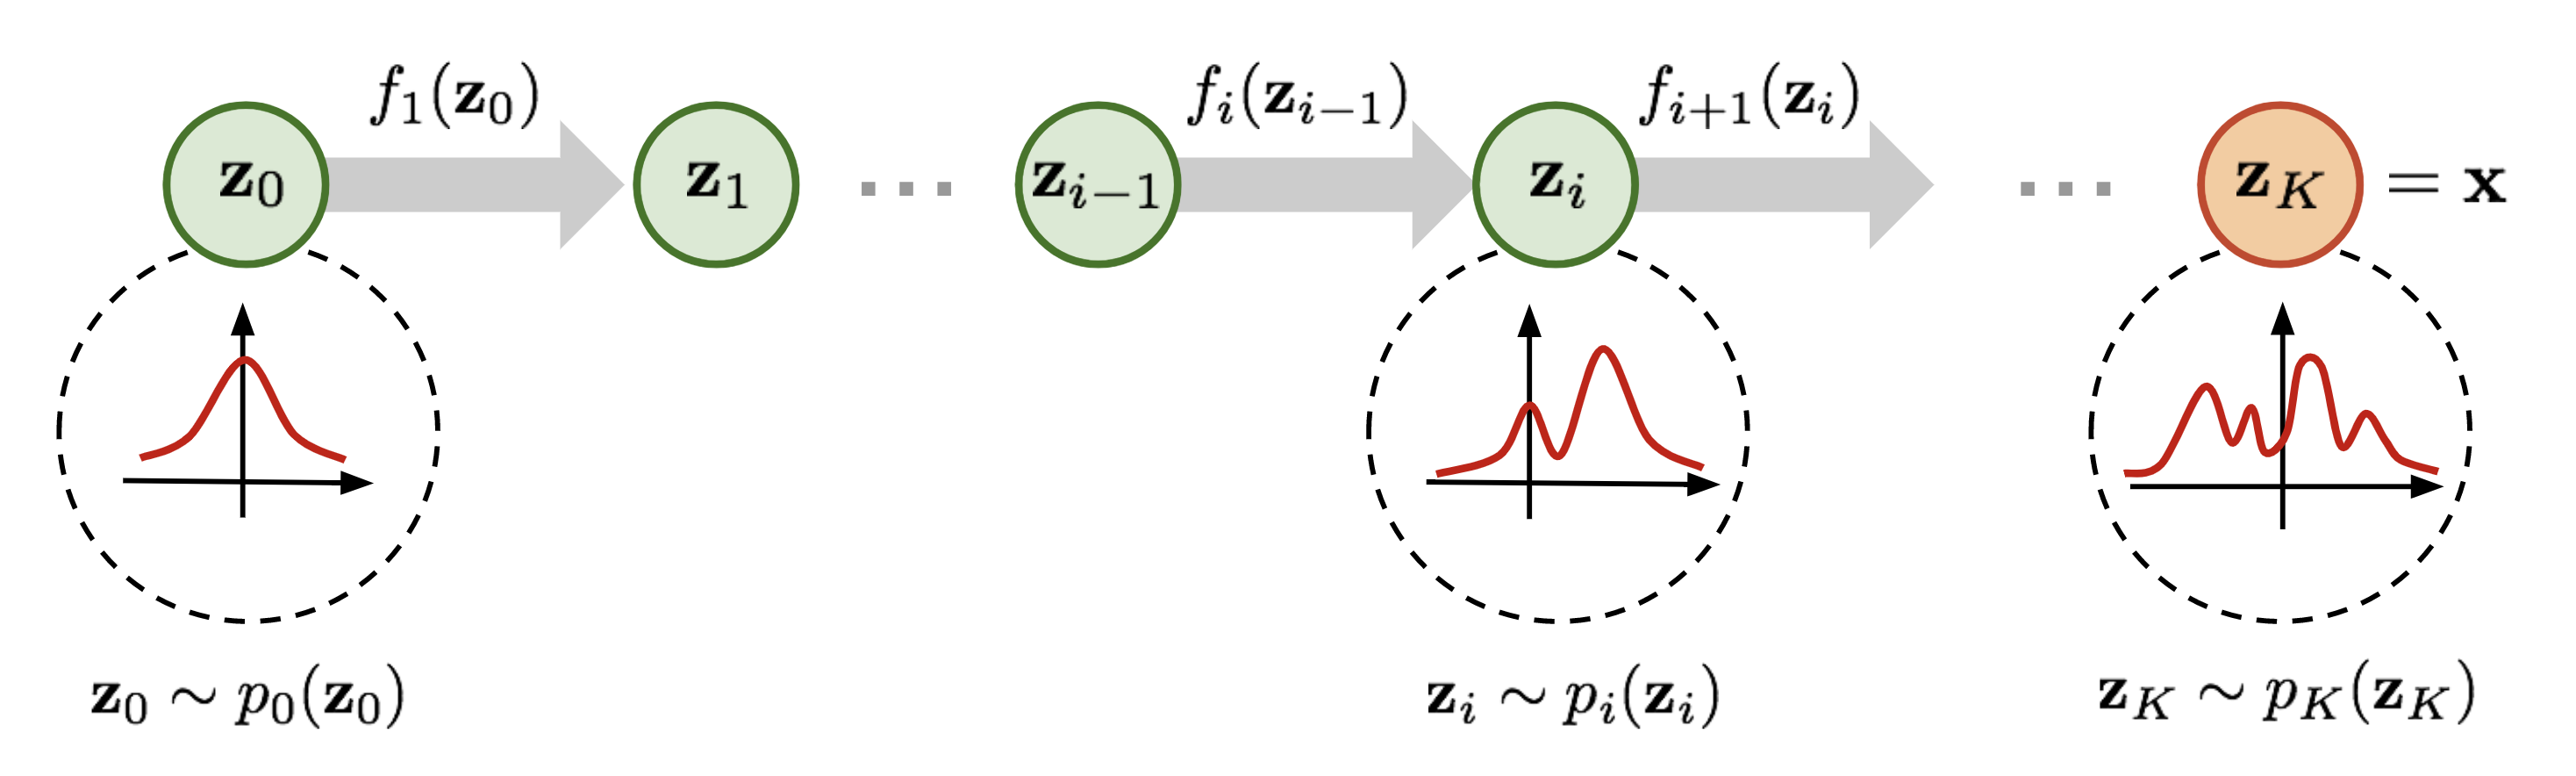
\includegraphics[width=0.4\textwidth]{figs/normalizing_flow_layout.png}
	\caption{ Schemata of "flow" from the base distribution $r(z)$ to $q(x)$
		\label{fig:schemaFlow}. \cite{nfSchema}
	}
\end{figure}


\subsection{training the transformation}
In order to receive a distribution $q(x)$ that represents the target distribution $p(x)$ closely we have to vary the parameters $\theta$ of the transformation $f$. One can use gradient descent with a divergence as a loss function. In this implementation the Kullback-Leibler (KL) divergence is used as one of the most popular.

In this case where we have samples of the target distribution it is suitable to work with the forward KL divergence between $p(x)$ and $q(x|\theta)$:

\begin{align*}
	\mathcal{L}(\theta) &= D_{KL}\left[p(x)\middle\|q(x|\theta)\right]\\
	&=-\mathbb{E}_{p(x)}\left[\ln(q(x|\theta))\right] + \text{const} \\
	&\approx -\frac{1}{N}\sum_{n=1}^{N}\ln(r(f^{-1}(x_n|\theta))) + \ln\left|\text{det}J_{f^{-1}}(x_n|\theta)\right| + \text{const}
\end{align*} 

where the $x_n$ are the sampled target data. Thus we have to be able to compute $f^{-1}$, its jacobian determinant and evaluate $r(z)$ and since we want do use gradient descend we need to differentiate through them. \cite{LuRi}

\section{Normalizing flow categories}
The two normalizing flow parameterizations we used are a Masked Autoencoder (\textbf{MADE}) \cite{pmlr-v37-germain15}, provided by the tensorflow library and a Real NVP \cite{JMLR:v22:19-1028}. 
The transformation of the Real NVP is:
\begin{align*}
	x_{0...\frac{d-1}{2}} &\rightarrow \alpha \cdot x_{0...\frac{d-1}{2}} + \beta\\
	x_{\frac{d-1}{2}...d-1} &\rightarrow x_{\frac{d-1}{2}...d-1} \\
	\alpha &= s(x_{\frac{d-1}{2}...d-1}) \hspace{1cm} \beta = s(x_{\frac{d-1}{2}...d-1})
\end{align*}
where $d$ is the number of features and $s$ is a fully connected neural net with \textit{ReLU} activation functions. The last layer of the scale $\alpha$ is activated with $\tanh$ while the shift $\beta$ is linear activated.
Then the Jacobian determinant is:
\begin{align*}
	\ln\left|\text{det}J_{f_{k}^{-1}}(x_{k-1})\right| = \sum_{i=0}^{\frac{d}{2}} \ln(\alpha_i)
\end{align*}
Between these transformations we apply the permutation (0123) of the features.




\section{Methods}
We use the tensorflow library to build the normalizing flows. Especially essential are the bijector and distribution classes of the probability module.
We split the data into signal and background, and further into training, testing and validation subsets.
These contain 80\%, 10\% and 10\% of the data. The training data is divided into batches.
As the base distribution $r(z)$ we choose a multidimensional normal distribution.
The transformation is implemented as a \textit{ tensorflow Chain} of \textit{ tensorflow bijectors}. These bijectors are the coupling layers and the permutation from section \ref{sec:param trafo}.  
All bijectors have methods for computing the forward transformation, inverse of the transformation and the logarithmic Jacobian determinate.

For training the flow we iterate over all batches and apply the gradient of the loglikelihood with the adams optimizer using \textit{tensorflow GradientTape}. The learning rate decays from a set initial value to a set final value with a polynomial decay with power $\frac{1}{2}$.
We train the models until the relative change of the loss function on the testing data is bellow \SI{1e-6}.
We oriented us closely to \cite{LuRi}.

For evaluating the validity of the model we calculate the test statistic $t$ from section \ref{sec:theory 1}, also we calculate the fraction of correctly classified data from the validation data given some cut and we look at the ROC-Curve of the test statistic.

\section{Results}
We first trained the models on default parameters, listed in table \ref{tab: defparams}. Since the number of background entries and signal entries differ greatly we used different batchsizes. The cut specifies at which value of the test statistic $t$ we classify a data point as background or signal. Layers determines how many coupling layers and permutations make up the model. There are also model specific parameters which control the shape of the \textbf{ANN}s.


\begin{table}
	\centering
	\begin{tabular}{|l|l|l|l|}
		\hline  
		\multicolumn{2}{|c|}{\textbf{parameter}}&	\multicolumn{2}{c|}{\textbf{value}} \\
		\hline
		\multicolumn{2}{|c|}{batchsize 0}&	\multicolumn{2}{c|}{1000} \\
		\hline
		\multicolumn{2}{|c|}{batchsize 1}&	\multicolumn{2}{c|}{100} \\
		\hline
		\multicolumn{2}{|c|}{cut}&	\multicolumn{2}{c|}{0} \\
		\hline
		\multicolumn{2}{|c|}{start learningrate}&	\multicolumn{2}{c|}{\SI{1e-3}} \\
		\hline
		\multicolumn{2}{|c|}{final learningrate}&	\multicolumn{2}{c|}{\SI{1e-4}} \\
		\hline
		\multicolumn{2}{|c|}{layers}&	\multicolumn{2}{c|}{8} \\
		\hline
		\hline
		\multicolumn{2}{|c|}{\textbf{MADE}} & \multicolumn{2}{c|}{\textbf{Real NVP}}\\
		\hline
		nodes per hidden layer & 200 & nodes per hidden layer & 100\\
		\hline
		number of hidden layers& 2 & number of hidden layers & 4\\
		\hline
	\end{tabular}
	\caption{Default parameters for the normalizing flow models and training \label{tab: defparams}}
\end{table}

Both models result in histograms of the test statistic as in \ref{fig:histt}
 \begin{figure*}[ht]
	\centering
	\begin{subfigure}[h]{0.475\textwidth}
		\centering
		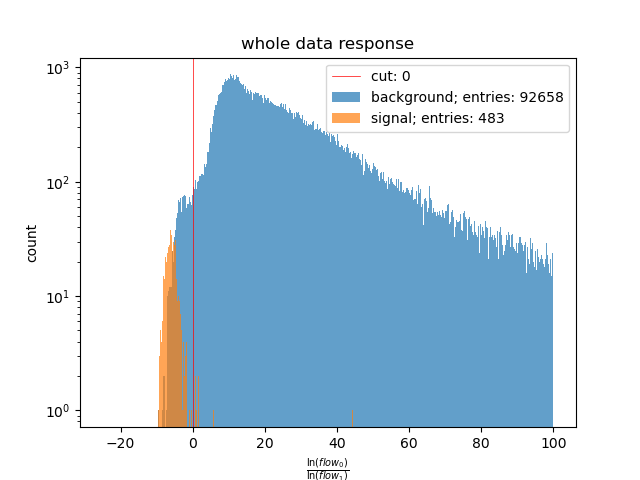
\includegraphics[width=\textwidth]{figs/fracln_data_hist_Real_NVP.png}
		%\caption[feature $u-g$ of the data]%
		%{{\small Network 1}}    
	\end{subfigure}
	\hfill
	\begin{subfigure}[h]{0.475\textwidth}  
		\centering 
		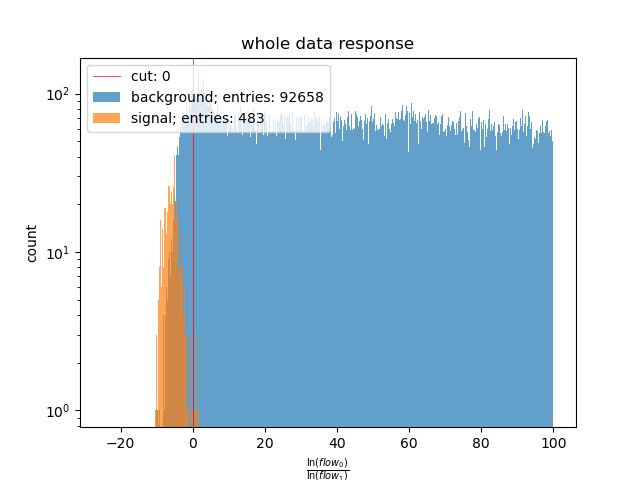
\includegraphics[width=\textwidth]{figs/fracln_data_hist_MADE.png}
		%\caption[]%
		%{{\small Network 2}}    
	\end{subfigure}
	\caption[ histograms of the test statistic $t$ for (left) Real NVP (right) MADE ]
	{\small histograms of the test statistic $t$ for (left) Real NVP (right) MADE} 
	\label{fig:histt}
\end{figure*}
We can see that both models deliver a negative response for the signal. For the background we observe that most of the data has a positive test statistic $t$, thus a classification of signal and background with a cut at $t=0$ is the best cut to minimize false negative classification, but there is also background data, that has $t<0$. With a cut of 0 the results of the classification are shown in table \ref{tab: res}, with : 
\begin{align*}
\text{correctly classified}~&=~\frac{\# \text{true positive}+ \# \text{true negative}}{\# \text{all}}\\ \text{false positive}~&=~\frac{\# \text{false positive}}{\# \text{all}}\\
\text{false negative}~&=~\frac{\# \text{false negative}}{\# \text{all}}
\end{align*}
Both models classify 98\% of the data correctly, leaving only 1\% false positive results.
 In figure \ref{fig:ROC} we see the ROC-Curves for both models. Since the false positive and the false negative rates are low the ROC-Curves show very high efficiency for low error rates, thus stating that the chosen cut has little impact.
\begin{table}
	\centering
	\begin{tabular}{|l|l|l|}
		\hline
		& Real NVP& MADE \\
		\hline
		correctly classified & 0.9870  & 0.9831\\
		\hline
		false positive &0.0126 & 0.0166 \\
		\hline
		false negative &0.0003 & 0.0002\\
		\hline
	\end{tabular}
	\caption{Results of the classification for Real NVP and MADE. \label{tab: res}}
\end{table}

 \begin{figure*}[ht]
	\centering
	\begin{subfigure}[h]{0.4\textwidth}
		\centering
		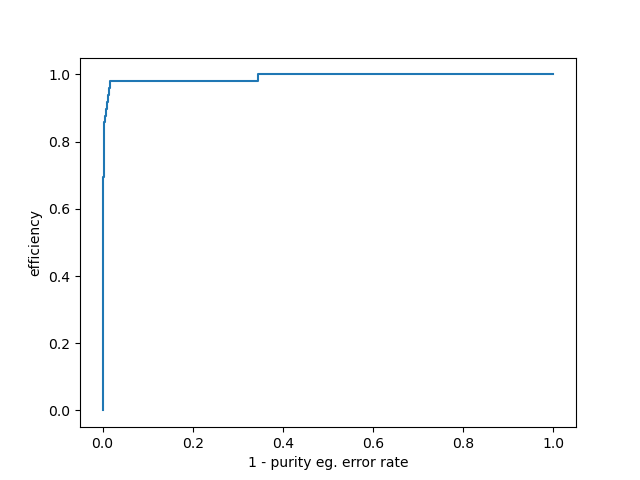
\includegraphics[width=\textwidth]{figs/ROC_validation_Real_NVP.png}
		%\caption[feature $u-g$ of the data]%
		%{{\small Network 1}}    
	\end{subfigure}
	\hfill
	\begin{subfigure}[h]{0.4\textwidth}  
		\centering 
		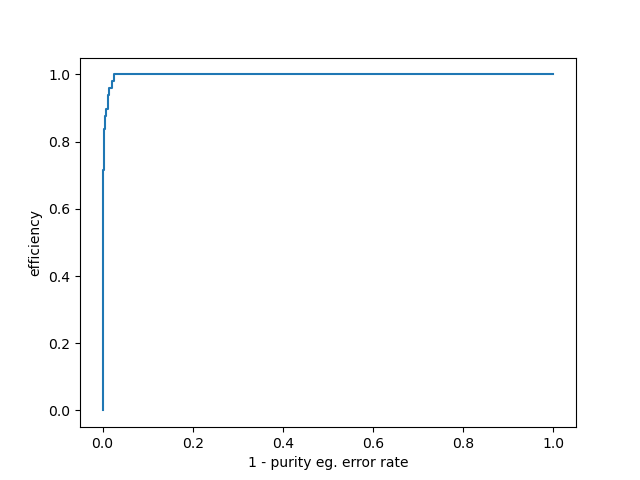
\includegraphics[width=\textwidth]{figs/ROC_validation_MADE.png}
		%\caption[]%
		%{{\small Network 2}}    
	\end{subfigure}
	\caption[ ROC-Curve of the Real NVP (left) and MADE (right)]
	{\small ROC-Curve of the Real NVP (left) and MADE (right)} 
	\label{fig:ROC}
\end{figure*}

In figure \ref{fig:losst} we see the loss of the Real NVP during training. Since the data of the background is fare greater than of the signal the number of needed steps for training the 0 flow is much less than of the signal. Since the loss function has a constant offset the loss during training does not approach 0. We can also see that the loss of the signal flow 1 is less smooth than of flow 0, because of the different batch sizes.

 \begin{figure*}[ht]
	\centering
	\begin{subfigure}[h]{0.4\textwidth}
		\centering
		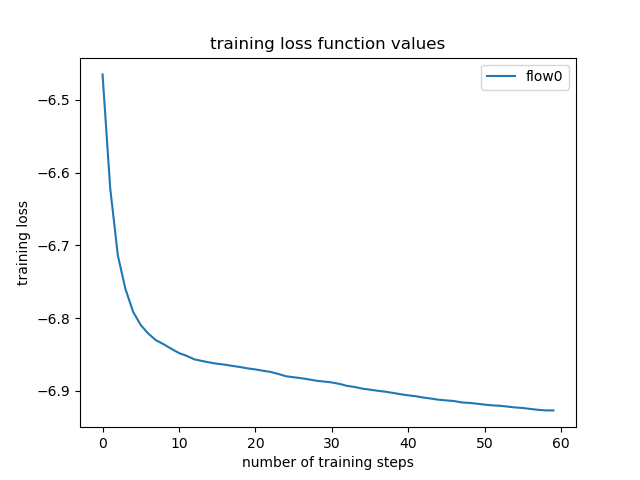
\includegraphics[width=\textwidth]{figs/training_loss_0_Real_NVP.png}
		%\caption[feature $u-g$ of the data]%
		%{{\small Network 1}}    
	\end{subfigure}
	\hfill
	\begin{subfigure}[h]{0.4\textwidth}  
		\centering 
		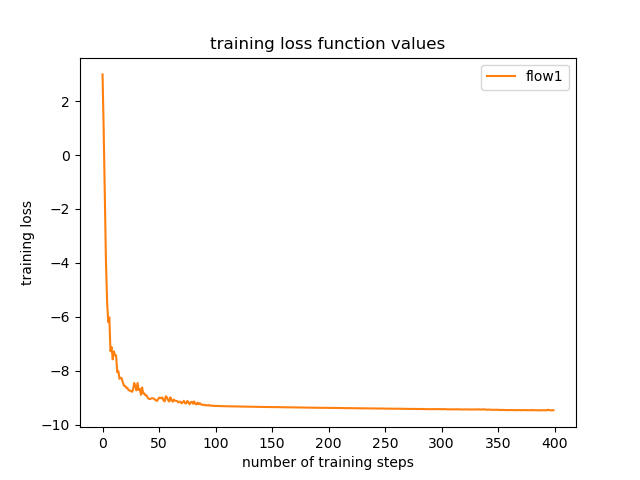
\includegraphics[width=\textwidth]{figs/training_loss_1_Real_NVP.png}
		%\caption[]%
		%{{\small Network 2}}    
	\end{subfigure}
	\caption[ loss function over time on the training data of the Real NVP]
	{\small loss function over time on the training data of the Real NVP} 
	\label{fig:losst}
\end{figure*}


\section{Conclusion}
The normalizing flow method for classification of RR-Lyrae stars is successful, achieving correct classification of 98\% . Two normalizing flow models are implemented, using the tensorflow library and tested, showing little difference on the giving data set. 


\bibliography{report}
%
%\section{\label{sec:level1}First-level heading}
%
%This sample document was adapted from the template for papers
%in APS journals.
%It demonstrates proper use of REV\TeX~4.1 (and
%\LaTeXe) in mansucripts prepared for submission to APS
%journals. Further information can be found in the REV\TeX~4.1
%documentation included in the distribution or available at
%\url{http://authors.aps.org/revtex4/}.
%
%When commands are referred to in this example file, they are always
%shown with their required arguments, using normal \TeX{} format. In
%this format, \verb+#1+, \verb+#2+, etc. stand for required
%author-supplied arguments to commands. For example, in
%\verb+\section{#1}+ the \verb+#1+ stands for the title text of the
%author's section heading, and in \verb+\title{#1}+ the \verb+#1+
%stands for the title text of the paper.
%
%Line breaks in section headings at all levels can be introduced using
%\textbackslash\textbackslash. A blank input line tells \TeX\ that the
%paragraph has ended. Note that top-level section headings are
%automatically uppercased. If a specific letter or word should appear in
%lowercase instead, you must escape it using \verb+\lowercase{#1}+ as
%in the word ``via'' above.
%
%\subsection{\label{sec:level2}Second-level heading: Formatting}
%
%This file may be formatted in either the \texttt{preprint} or
%\texttt{reprint} style. \texttt{reprint} format mimics final journal output.
%Either format may be used for submission purposes. \texttt{letter} sized paper should
%be used when submitting to APS journals.
%
%\subsubsection{Wide text (A level-3 head)}
%The \texttt{widetext} environment will make the text the width of the
%full page, as on page~\pageref{eq:wideeq}. (Note the use the
%\verb+\pageref{#1}+ command to refer to the page number.)
%\paragraph{Note (Fourth-level head is run in)}
%The width-changing commands only take effect in two-column formatting.
%There is no effect if text is in a single column.
%
%\subsection{\label{sec:citeref}Citations and References}
%A citation in text uses the command \verb+\cite{#1}+ or
%\verb+\onlinecite{#1}+ and refers to an entry in the bibliography.
%An entry in the bibliography is a reference to another document.
%
%\subsubsection{Citations}
%Because REV\TeX\ uses the \verb+natbib+ package of Patrick Daly,
%the entire repertoire of commands in that package are available for your document;
%see the \verb+natbib+ documentation for further details. Please note that
%REV\TeX\ requires version 8.31a or later of \verb+natbib+.
%
%\paragraph{Syntax}
%The argument of \verb+\cite+ may be a single \emph{key},
%or may consist of a comma-separated list of keys.
%The citation \emph{key} may contain
%letters, numbers, the dash (-) character, or the period (.) character.
%New with natbib 8.3 is an extension to the syntax that allows for
%a star (*) form and two optional arguments on the citation key itself.
%The syntax of the \verb+\cite+ command is thus (informally stated)
%\begin{quotation}\flushleft\leftskip1em
%  \verb+\cite+ \verb+{+ \emph{key} \verb+}+, or\\
%  \verb+\cite+ \verb+{+ \emph{optarg+key} \verb+}+, or\\
%  \verb+\cite+ \verb+{+ \emph{optarg+key} \verb+,+ \emph{optarg+key}\ldots \verb+}+,
%\end{quotation}\noindent
%where \emph{optarg+key} signifies
%\begin{quotation}\flushleft\leftskip1em
%  \emph{key}, or\\
%  \texttt{*}\emph{key}, or\\
%  \texttt{[}\emph{pre}\texttt{]}\emph{key}, or\\
%  \texttt{[}\emph{pre}\texttt{]}\texttt{[}\emph{post}\texttt{]}\emph{key}, or even\\
%  \texttt{*}\texttt{[}\emph{pre}\texttt{]}\texttt{[}\emph{post}\texttt{]}\emph{key}.
%\end{quotation}\noindent
%where \emph{pre} and \emph{post} is whatever text you wish to place
%at the beginning and end, respectively, of the bibliographic reference
%(see Ref.~[\onlinecite{witten2001}] and the two under Ref.~[\onlinecite{feyn54}]).
%(Keep in mind that no automatic space or punctuation is applied.)
%It is highly recommended that you put the entire \emph{pre} or \emph{post} portion
%within its own set of braces, for example:
%\verb+\cite+ \verb+{+ \texttt{[} \verb+{+\emph{text}\verb+}+\texttt{]}\emph{key}\verb+}+.
%The extra set of braces will keep \LaTeX\ out of trouble if your \emph{text} contains the comma (,) character.
%
%The star (*) modifier to the \emph{key} signifies that the reference is to be
%merged with the previous reference into a single bibliographic entry,
%a common idiom in APS and AIP articles (see below, Ref.~[\onlinecite{epr}]).
%When references are merged in this way, they are separated by a semicolon instead of
%the period (full stop) that would otherwise appear.
%
%\paragraph{Eliding repeated information}
%When a reference is merged, some of its fields may be elided: for example,
%when the author matches that of the previous reference, it is omitted.
%If both author and journal match, both are omitted.
%If the journal matches, but the author does not, the journal is replaced by \emph{ibid.},
%as exemplified by Ref.~[\onlinecite{epr}].
%These rules embody common editorial practice in APS and AIP journals and will only
%be in effect if the markup features of the APS and AIP Bib\TeX\ styles is employed.
%
%\paragraph{The options of the cite command itself}
%Please note that optional arguments to the \emph{key} change the reference in the bibliography,
%not the citation in the body of the document.
%For the latter, use the optional arguments of the \verb+\cite+ command itself:
%\verb+\cite+ \texttt{*}\allowbreak
%\texttt{[}\emph{pre-cite}\texttt{]}\allowbreak
%\texttt{[}\emph{post-cite}\texttt{]}\allowbreak
%\verb+{+\emph{key-list}\verb+}+.

\end{document}
%
% ****** End of file templateForReport.tex ******
